\chapter{Cwiczenie 3}

\section{Zjawisko dudnień}

\begin{itemize}
    \item Wykonano sumowanie dwóch sygnałów sinusoidalnych o skrajnie bliskich częstotliwościach i jednakowych amplitudach za pomocą opcji oscyloskopu - \textbf{Math} (czerwony przycisk znajdujący się obok przycisków kanałów.
    \item Przyjęte wartości, odpowiednio \textbf{kanał 1}, \textbf{kanał 2} - (1kHz, 1V), (1.05kHz, 1V)
\end{itemize}

\section{Wypadkowa częstotliwość}

\begin{itemize}
    \item Teoretyczna wypadkowa częstotliwość przyjmuje wartość:
    \begin{equation}
        f_{wyp} = \frac{f_1 + f_2}{2} = \frac{2.05kHz}{2} = 1.025kHz = \textbf{1025Hz}
    \end{equation}
    \begin{center}
        Zmierzona wartość wyniosła 1.02kHz = \textbf{1020Hz}
    \end{center}
    \begin{center}
        \label{ad:roznica_4_2-1}
        \textcolor{purple}{Różnica $\Delta$ = $f_{wyp}$ - $f_{zmierzona}$ =} \textbf{5Hz}
    \end{center}
    \begin{figure}[h]
        \centering
        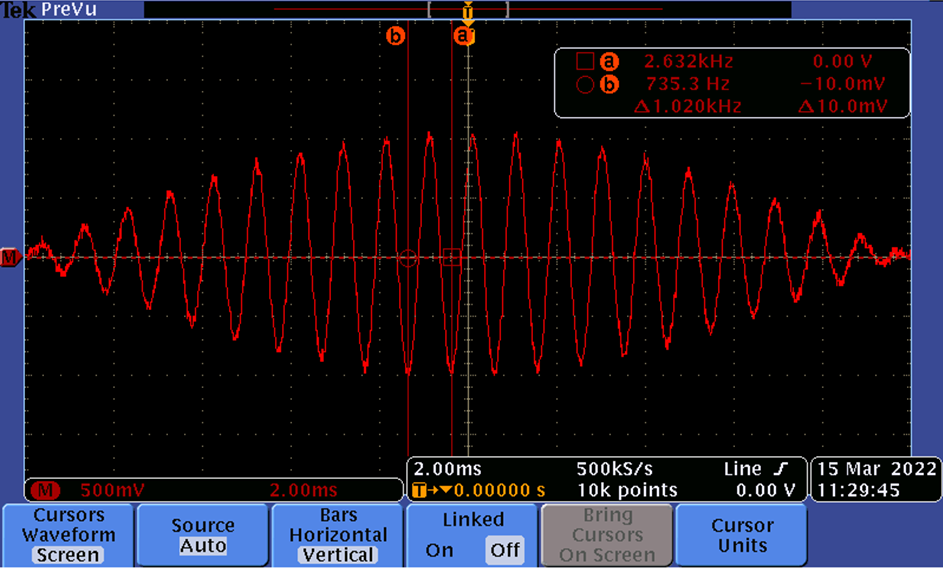
\includegraphics[scale=1.4]{images/srednia_czestotliwosc.png}
        \caption{Wypadkowa częstotliwość zmierzona za pomocą kursorów}
        \label{fig:wypadkowa}
    \end{figure}
\end{itemize}

\section{Częstotliwość dudnienia}
    
\begin{itemize}
    \item Częstotliwość dudnienia zmierzono za pomocą kursorów. Przewidywana wartość wynosiła:
    \begin{equation}
        f_{dud} = |f_1 - f_2| = 0.05kHz = \textbf{50Hz}
    \end{equation}
    Zmierzona wartość wyniosła \textbf{50Hz}
    \begin{figure}[h]
        \centering
        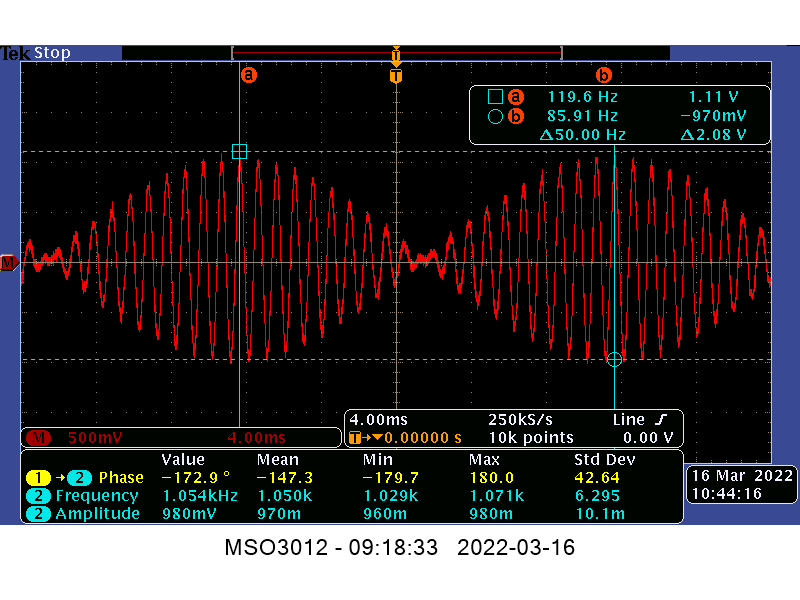
\includegraphics[scale=0.33]{images/1_6-okresdudnien.png}
        \caption{Pomiar częstotliwości dudnień za pomocą kursorów}
        \label{fig:cz_dudnienia}
    \end{figure}
    
\section{Częstotliwość modulacji}
    
    \item Teoretyczna wartość częstotliwości modulacji:
    \begin{equation}
        f_{mod} = \frac{|f_1 - f_2|}{2} = \textbf{25Hz}
    \end{equation}
    Zmierzona wartość wyniosła \textbf{25.25Hz}. Różnica wyniosła $\approx$ \textbf{0.25Hz}
    \begin{figure}[h]
        \centering
        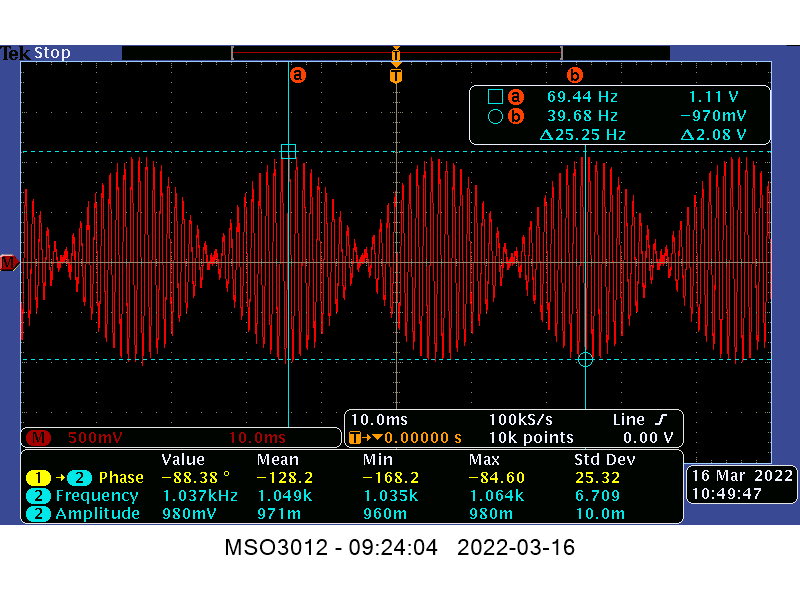
\includegraphics[scale=0.33]{images/1_6-okresmodulacji.png}
        \caption{Pomiar częstotliwości modulacji za pomocą kursorów}
        \label{fig:cz_modulacji}
    \end{figure}
\end{itemize}

\section {Podsumowanie}

\begin{itemize}
    \item Uzyskane pomiary za pomocą kursorów były bardzo zbliżone do teoretycznych wyliczeń
    \item Pomiary zarówno wypadkowej częstotliwości jak i częstotliwości dudnień oraz modulacji nie przekraczały błędu względnego (względem teoretycznej wartości) 1\%
    \item Różnica w uzyskanych wynikach spowodowana jest przez niedokładność pomiarów z użyciem kursorów
\end{itemize}